\documentclass[../main.tex]{subfiles}
\begin{document}


\subsection{Dihedral groups}

The dihedral group, $D_{2n}$, is the group of symmetries of a regular n-gon. Its standard presentation is given by
\[
\abr{r,s \ \middle| \  r^n = s^2 = e, \ (rs)^2 = e}
\]
where r is a rotation of $2\pi/n$ and s is a reflection.\\

Let $l_{1}$ and $l_{2}$ be two reflection axes with an angle $\theta$ between $l_{1}$ and $l_{2}$, and $s_{1}$ and $s_{2}$ be the respective reflections. After some algebra, the composition $s_{1}s_{2}$ turns out to be a counterclockwise rotation through $2\theta$.\\

Therefore, an alternative presentation of $D_{2n}$ is given by
\[
\abr{s_1,s_2 \ \middle| \ s_1^2 = s_2^2 = e, \ (s_1s_2)^n = e}
\]
where $s_{1}$ and $s_{2}$ are adjacent reflections.\\

This shows that $D_{2n}$ is an example of a reflection group.

\begin{figure}[ht]
    \centering
    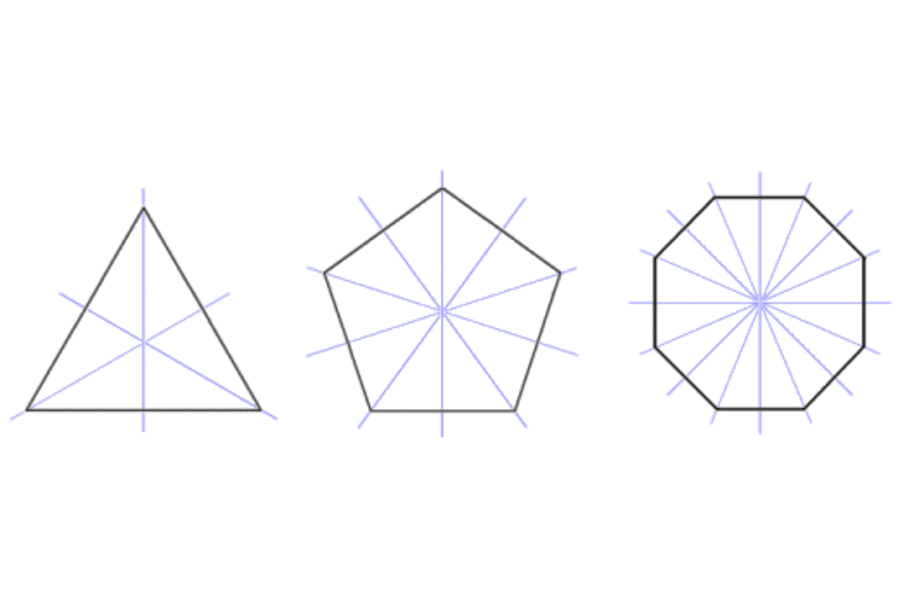
\includegraphics[width=0.5\textwidth]{polygons.pdf}
    \caption{The lines of symmetry of a regular 3-,4- and 7-gon.}
    \label{}
\end{figure}

\begin{example}
The coxeter diagram for the symmetries of a regular n-gon, also known as $I_{2}(n)$, looks like
    \begin{figure}[H]
    \centering
    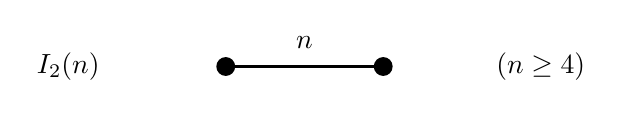
\begin{tikzpicture}
        \begin{scope}[shift={(0,-21.5)}]
        \node at (0,0) {$I_2(n)$};
        \begin{scope}[every node/.style={circle, fill=black, draw, thick, minimum size = 6pt, inner sep=0pt}]
            \node (1) at (2,0) {};
            \node (2) at (4,0) {};
        \end{scope}
        \begin{scope}[every edge/.style={draw,very thick}]
            \path [-] (1) edge (2);
            \node at (3,0.3) {$n$};
            \node at (6,0) {$(n\geq 4)$};
        \end{scope}
    \end{scope}
\end{tikzpicture}

\end{figure}
\end{example}


\begin{theorem}[]
\label{}
Let \( G \curvearrowright X \) be an action of a finite group \( G \) on a finite set \( X \).  
Then the number of \( G \)-orbits in \( X \) is given by:
\[
\text{Number of orbits} = \frac{1}{|G|} \sum_{g \in G} |\mathrm{Fix}(g)|
\]
where \( \mathrm{Fix}(g) = \{ x \in X \mid g \cdot x = x \} \).
\end{theorem}

\begin{example}\cite{fraleigh}
How many distinguishable necklaces can be made using seven different colored beads of the same size?\\
    Let X be the $7!$ possible arrangements. The necklace can be turned over (a reflection) as well as rotated so we consider the dihedral group $D_{14}$ acting on X. Using the previous theorem, 
\[
\text{Number of orbits} = \frac{7!}{14}\ = 360
\]
as only the identity leaves any arrangement fixed.
\end{example}

\begin{theorem}
Let p be a prime. Then any group $G$ of order $2p$ is isomorphic to either the cyclic group $C_{2p}$ or the dihedral group $D_{2p}$.

\textbf{Proof}.  
By Cauchy's theorem, there exists an element \( a \in G \) of order $p$ and an element \( b \in G \) of order $2$. Let
\[
H = \langle a \rangle,
\]
so \( H \) is a subgroup of G of index 2, so \( H \trianglelefteq G \).

Since \( H \trianglelefteq G \), conjugation by \( b \) sends \( H \) to itself. Thus, there exists \( k \in \{1, 2, \ldots, p-1\} \) such that
\[
b a b^{-1} = a^k.
\]

Applying conjugation by \( b \) twice to \( a \) gives
\[
a = b^2 a b^{-2} = b (b a b^{-1}) b^{-1} = b a^k b^{-1} = (b a b^{-1})^k = (a^k)^k = a^{k^2}.
\]

Therefore,
\[
a = a^{k^2} \implies a^{k^2 - 1} = e.
\]

Since \( a \) has order \( p \), this implies
\[
p \mid (k^2 - 1),
\]
or equivalently,
\[
k^2 \equiv 1 \pmod p.
\]

Because \( p \) is prime, this implies
\[
k \equiv \pm 1 \pmod p.
\]

\begin{itemize}
\item If \( k \equiv 1 \), then
\[
b a b^{-1} = a,
\]
and \( b \) commutes with \( a \). Hence \( G \) is abelian, and since \( a \) has order \( p \) and \( b \) has order 2, \( G \) is cyclic of order \( 2p \).

\item If \( k \equiv -1 \), then
\[
b a b^{-1} = a^{-1},
\]
which is the defining relation for the dihedral group \( D_{2p} \):
\[
D_p = \langle a, b \mid a^p = e, b^2 = e, b a b = a^{-1} \rangle.
\]
\end{itemize}

Thus, \( G \) is isomorphic to either \( C_{2p} \) or \( D_{2p} \).

\hfill\(\Box\)
\end{theorem}

\subsection{The Infinite dihedral group}

We can also consider the group generated by two reflections $s_1,s_2$ with order of $s_1s_2$ infinite. This is the infinite dihedral group denoted by $D_{\infty}$. Note every finite dihedral group is a quotient group of $D_{\infty}$. The quotient map is simply sending generators to generators. $D_{\infty}$ can be taken as the symmetry group of the real line, with all integers distinguished. \textcolor{red}{Add a picture?} 
The generators can be any two consecutive distinguished points on that line. This is an example of affine reflection groups we will define later, and also the simplest example. 






\section{Platonic solids and reflections}
\begin{figure}[ht]
    \centering
    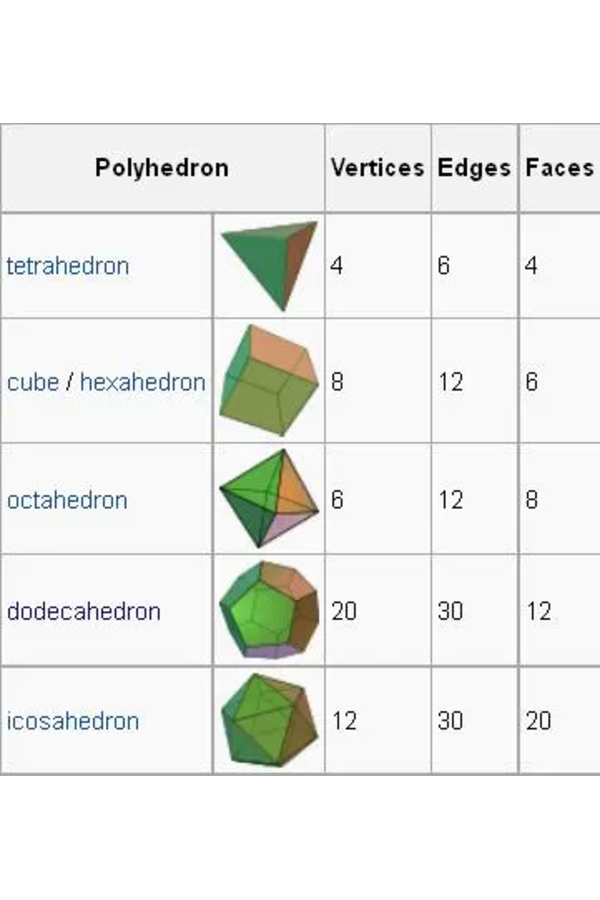
\includegraphics[width=0.4\textwidth]{platonic solids.pdf}
    \caption{The five Platonic solids.}
    \label{platonic solids}
\end{figure}

\begin{definition}
    A polyhedron is regular if its faces are regular polygons, all with the same number of sides, and also each vertex belongs to the same number of edges.
\end{definition}

\begin{theorem}
The only regular convex polyhedra are the five Platonic solids.\\
\textbf{Proof}. Before writing the proof, we introduce some notations.\\
$V$, the number of vertices;\\
$E$, the number of edges;\\
$F$, the number of faces;\\
$n$, the number of sides on a face;\\
$r$, the number of edges to which each vertex belongs.\\
Observe that 
\begin{equation}\label{eqn_1}
2E=nF
\end{equation}
and
\begin{equation}\label{eqn_2}
2E=rV
\end{equation}
(1) comes from counting the number of pairs (e,f) where e is an edge and f is a face and e lies on f; (2) comes from counting the number of pairs (v,e) where v is a vertex and v lies on e.\\
Substitute into Euler's formula, we get 
\begin{equation}\label{eqn_3}
\frac{1}{r}+\frac{1}{n}=\frac{1}{2}+\frac{1}{E}
\end{equation}
Now $n\geq 3$, as a polygon must have at least $3$ sides and $r\geq 3$, since in a polyhedron a vertex must belong to at least $3$ edges. By (3), we can't have both $n\geq 4$ and $r \geq 4$, since this would make the left-hand side of (3) at most $\frac{1}{2}$.
It follows that either $n = 3$ or $r = 3$.
If $n = 3$, then (3) becomes
\begin{equation}\label{eqn_4}
\frac{1}{r}=\frac{1}{6}+\frac{1}{E}
\end{equation}
The right-hand side is greater than $\frac{1}{6}$, and hence $r < 6$. Therefore, $r = 3$, $4$ or $5$ and $E = 6$, $12$ or $30$, respectively.
If $r = 3$, (3) becomes
\begin{equation}\label{eqn_5}
\frac{1}{n}=\frac{1}{6}+\frac{1}{E}
\end{equation}
Similarly, n = 3,4 or 5 and E = 6,12 or 30, respectively.
These parameters coincide with those in the table above.
\hfill\(\Box\)
\end{theorem}

\begin{example}
Let $G$ be the group of symmetries of a dodecahedron. What is $|G|$?\\
Let G act on the 12 faces of the dodecahedron and fix a face. There are $|D_{10}|=10$ symmetries which fix this face and our action is clearly transitive. By Orbit-Stabiliser theorem, $|G|=10\times12=120.$
Alternatively, this can be done by considering the fundamental domain, which is a triangle that uniquely determines the reflection. There are 120 such triangles.
\end{example}



We would like to study the group of symmetries of these Platonic solids.

\subsection{Cube}
We start by investigating the cube.


\tdplotsetmaincoords{60}{30}
\begin{center}
\begin{tikzpicture}[tdplot_main_coords, scale=1.5]

\draw[->] (0,0,0) -- (2.5,0,0) node[anchor=north east]{$x$};
\draw[->] (0,0,0) -- (0,3,0) node[anchor=south east]{$y$};
\draw[->] (0,0,0) -- (0,0,2.5) node[anchor=south]{$z$};


\def\s{1}


\draw[thick] (-\s,-\s,-\s) -- (\s,-\s,-\s) -- (\s,\s,-\s) -- (-\s,\s,-\s) -- cycle;

\draw[thick] (-\s,-\s,\s) -- (\s,-\s,\s) -- (\s,\s,\s) -- (-\s,\s,\s) -- cycle;

\foreach \x in {-1,1} {
  \foreach \y in {-1,1} {
    \draw[thick] (\x,\y,-1) -- (\x,\y,1);
  }
}

\draw[->, thick, red] (0,0,0) -- (1,0,0) node[below right] {$\mathbf{u}=(1,0,0)$};
\draw[->, thick, blue] (0,0,0) -- (1,1,0) node[below right] {$\mathbf{v}=(1,1,0)$};
\draw[->, thick, green!60!black] (0,0,0) -- (0,1,1) node[left] {$\mathbf{w}=(0,1,1)$};

\node[below left] at (0,0,0) {\(O\)};
\end{tikzpicture}
\end{center}
As, seen before, $s_{\mathbf{u}}$ and $s_{\mathbf{v}}$ generates the square. It turns out that $s_{\mathbf{u}}=(0,1,1)$, orthorgonal to $s_{\mathbf{u}}$, is a clever third choice of vector, which gives $(s_{\mathbf{u}}s_{\mathbf{w}})^2=e$. Moreover, $\mathbf{u} \cdot \mathbf{w}=\frac{1}{2}$ so the angle between $\mathbf{u}$ and $\mathbf{w}$ is $\frac{\pi}{3}$, hence $(s_{\mathbf{u}}s_{\mathbf{w}})^3=e$. Thus the coxeter diagram for the symmetries of the cube, also known as $BC_{3}$, looks like
\begin{figure}[!h]
\centering
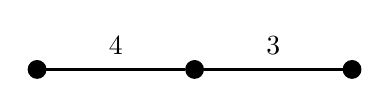
\begin{tikzpicture}
    \begin{scope}[every node/.style={circle, fill=black, draw, thick, minimum size = 6pt, inner sep=0pt}]
        \node (1) at (0,0) {};
        \node (2) at (2,0) {};
        \node (3) at (4,0) {};
    \end{scope}

    \begin{scope}[every edge/.style={draw,very thick}]
        \path [-] (1) edge (2);
        \path [-] (2) edge (3);
        \node at (1,0.3) {$4$};
        \node at (3,0.3) {$3$};
    \end{scope}
\end{tikzpicture}
\end{figure}

Equivalently, recall that this is equivalent to the group presentation
\[
\abr{s_1,s_2,s_3 \ \middle| \ s_1^2 = s_2^2 = s_3^2 = e, \ (s_1s_2)^4 = (s_2s_3)^3 = (s_1s_3)^2 = e}
\]

\subsection{Dual}
Before moving on to the other solids, we first introduce the concept of dual.
\begin{definition}
   The dual of a Platonic solid is a new Platonic solid where the faces and vertices are interchanged with those of the original. 
\end{definition}

\begin{remark}
    The tetrahedron is self-dual. The cube and the octahedron form a dual pair. The dodecahedron and the icosahedron form a dual pair.
\end{remark}
\begin{figure}[ht]
    \centering
    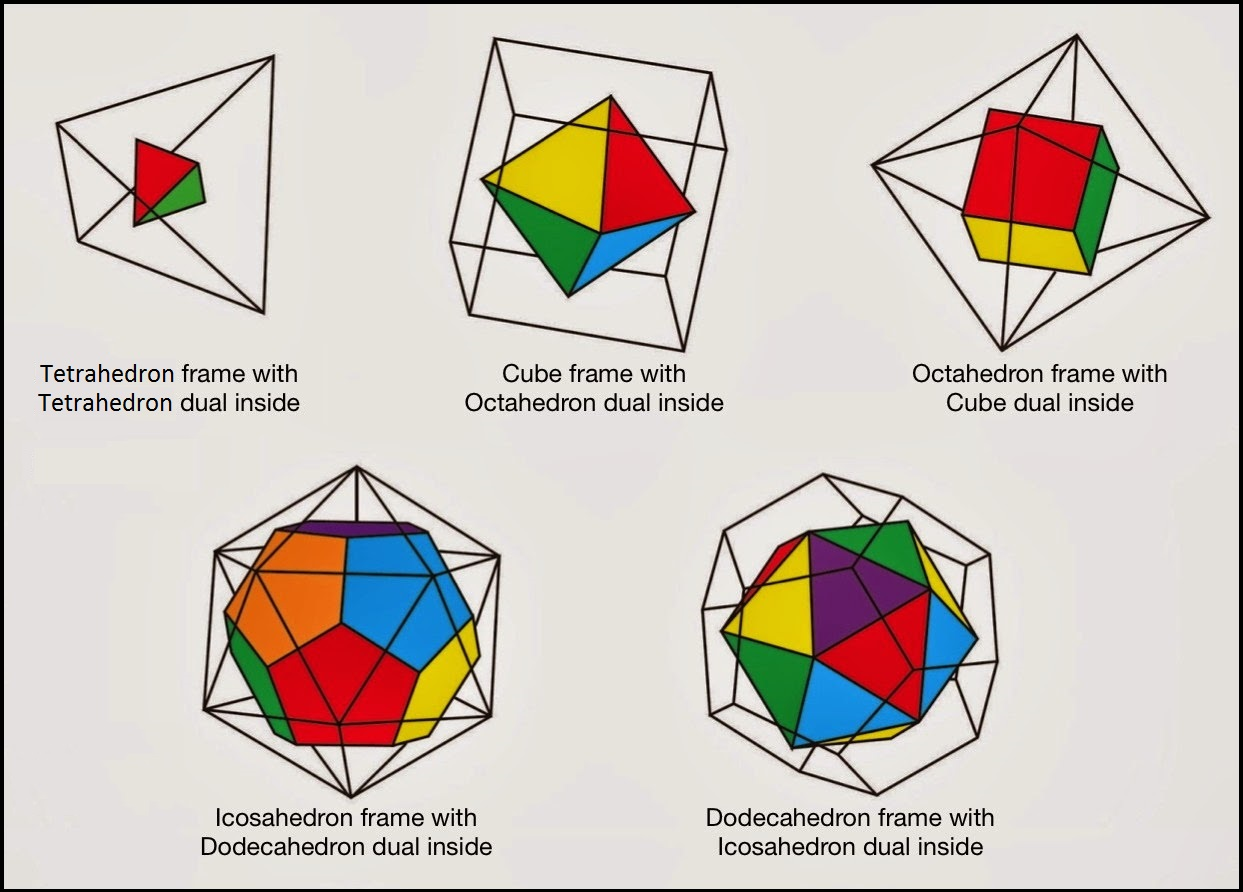
\includegraphics[width=0.4\textwidth]{PlatonicSolidsDual.jpg}
    \caption{Duals of each Platonic solid.}
    \label{}
\end{figure}

\begin{remark}
A polyhedron and its dual have the same axes of symmetry, so they have the same Coxeter diagram. For example, the Coxeter diagram for the symmetries of the octahedron is again $BC_{3}$ as seen before.   
\end{remark}

\subsection{Dodecahedron and isocahedron}

\begin{center}
\tdplotsetmaincoords{75}{115}
%
\begin{tikzpicture}[tdplot_main_coords,scale=1.75]
	\pgfmathsetmacro{\aureo}{0.5 * (1.0 + sqrt(5.0))} % the golden number
	\pgfmathsetmacro{\unidad}{1.0}
	\coordinate (1) at (0,\aureo,1);
	\coordinate (2) at (0,-\aureo,1);
	\coordinate (3) at (0,-\aureo,-1);
	\coordinate (4) at (0,\aureo,-1);
	\coordinate (5) at (1,0,\aureo);
	\coordinate (6) at (-1,0,\aureo);
	\coordinate (7) at (-1,0,-\aureo);
	\coordinate (8) at (1,0,-\aureo);
	\coordinate (9) at (\aureo,1,0);
	\coordinate (10) at (-\aureo,1,0);
	\coordinate (11) at (-\aureo,-1,0);
	\coordinate (12) at (\aureo,-1,0);


	% Hidden edges
	\draw[dashed,opacity=0.75] (6) -- (10);
	\draw[dashed,opacity=0.75] (6) -- (11);
	\draw[dashed,opacity=0.75] (10) -- (11);
	\draw[dashed,opacity=0.75] (2) -- (11);
	\draw[dashed,opacity=0.75] (3) -- (11);
	\draw[dashed,opacity=0.75] (7) -- (11);
	\draw[dashed,opacity=0.75] (7) -- (10);
	\draw[dashed,opacity=0.75] (4) -- (7);
	\draw[dashed,opacity=0.75] (3) -- (7);
	\draw[dashed,opacity=0.75] (8) -- (7);
	\draw[dashed,opacity=0.75] (2) -- (3);	

	
	% Visible edges
	\draw[thick,opacity=0.75] (5) -- (1);
	\draw[thick,opacity=0.75] (5) -- (2);
	\draw[thick,opacity=0.75] (5) -- (12);
	\draw[thick,opacity=0.75] (5) -- (9);
	\draw[thick,opacity=0.75] (5) -- (6);
	\draw[thick,opacity=0.75] (9) -- (4);
	\draw[thick,opacity=0.75] (9) -- (8);
	\draw[thick,opacity=0.75] (9) -- (1);
	\draw[thick,opacity=0.75] (6) -- (1);
	\draw[thick,opacity=0.75] (2) -- (12);
	\draw[thick,opacity=0.75] (9) -- (12);
	\draw[thick,opacity=0.75] (8) -- (12);
	\draw[thick,opacity=0.75] (4) -- (8);
	\draw[thick,opacity=0.75] (4) -- (1);
	\draw[thick,opacity=0.75] (2) -- (6);
	\draw[thick,opacity=0.75] (3) -- (12);
	\draw[thick,opacity=0.75] (8) -- (3);
	\draw[thick,opacity=0.75] (10) -- (1);
	\draw[thick,opacity=0.75] (4) -- (10);
	
    	
\draw[->] (0,0,0) -- (3,0,0) node[anchor=north east]{$x$};
\draw[->] (0,0,0) -- (0,2,0) node[anchor=south east]{$y$};
\draw[->] (0,0,0) -- (0,0,2) node[anchor=south]{$z$};

\draw[->, thick, red] (0,0,0) -- (1,0,0) node[below right] {$\mathbf{u}=(1,0,0)$};
\draw[->, thick, blue] (0,0,0) -- (1,1,0) node[below right] {$\mathbf{v}=(1,1,0)$};
\draw[->, thick, green!60!black] (0,0,0) -- (0,1,1) node[left] {$\mathbf{w}=(0,1,1)$};

\node[below left] at (0,0,0) {\(O\)};	

\end{tikzpicture}
\end{center}
The group presentation is
\[
\abr{s_1,s_2,s_3 \ \middle| \ s_1^2 = s_2^2 = s_3^2 = e, \ (s_1s_2)^3 = (s_2s_3)^5 = (s_1s_3)^2 = e}
\]

and the Coxeter diagram, also known as $H_{3}$, is
\begin{figure}[!h]
\centering
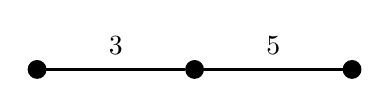
\begin{tikzpicture}
    \begin{scope}[every node/.style={circle, fill=black, draw, thick, minimum size = 6pt, inner sep=0pt}]
        \node (1) at (0,0) {};
        \node (2) at (2,0) {};
        \node (3) at (4,0) {};
    \end{scope}

    \begin{scope}[every edge/.style={draw,very thick}]
        \path [-] (1) edge (2);
        \path [-] (2) edge (3);
        \node at (1,0.3) {$3$};
        \node at (3,0.3) {$5$};
    \end{scope}
\end{tikzpicture}
\end{figure}
\subsection{Tetrahedron}

\tdplotsetmaincoords{70}{120}
\begin{center}
\begin{tikzpicture}[tdplot_main_coords, scale=2]

% Axes
\draw[->] (0,0,0) -- (2,0,0) node[anchor=north east]{$x$};
\draw[->] (0,0,0) -- (0,2,0) node[anchor=south east]{$y$};
\draw[->] (0,0,0) -- (0,0,2) node[anchor=south]{$z$};

% Shifted coordinates (origin at centroid)
\coordinate (A) at (3/2,-1/2,-1/2);
\coordinate (B) at (-1/2,3/2,-1/2);
\coordinate (C) at (-1/2,-1/2,3/2);
\coordinate (D) at (-1/2,-1/2,-1/2);

% Draw tetrahedron edges
\draw[thick] (A) -- (B) -- (C) -- (A);
\draw[thick] (D) -- (A);
\draw[thick] (D) -- (B);
\draw[thick] (D) -- (C);

% Root vectors
\draw[->, thick, red] (0,0,0) -- (1/2,-1/2,0) node[below right] {$\mathbf{u}=(1,-1,0)$};
\draw[->, thick, blue] (0,0,0) -- (0,1/2,-1/2) node[below right] {$\mathbf{v}=(0,1,-1)$};
\draw[->, thick, green!60!black] (0,0,0) -- (-1/2,0,1/2) node[left] {$\mathbf{w}=(-1,0,1)$};

\node[below left] at (0,0,0) {\(O\)};

\end{tikzpicture}
\end{center}


The group presentation is 
\[
\abr{s_1,s_2,s_3 \ \middle| \ s_1^2 = s_2^2 = s_3^2 = e, \ (s_1s_2)^3 = (s_2s_3)^3 = (s_1s_3)^2 = e}
\]
and the Coxeter diagram, also known as $A_{3}$ (careful, this is NOT the alternating group $A_{3}$), is
\begin{figure}[!h]
\centering
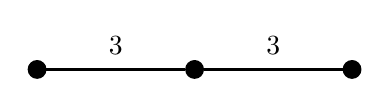
\begin{tikzpicture}
    \begin{scope}[every node/.style={circle, fill=black, draw, thick, minimum size = 6pt, inner sep=0pt}]
        \node (1) at (0,0) {};
        \node (2) at (2,0) {};
        \node (3) at (4,0) {};
    \end{scope}

    \begin{scope}[every edge/.style={draw,very thick}]
        \path [-] (1) edge (2);
        \path [-] (2) edge (3);
        \node at (1,0.3) {$3$};
        \node at (3,0.3) {$3$};
    \end{scope}
\end{tikzpicture}
\end{figure}

\end{document}